\par This section describes the variables used in the $\nu_e$ selections to isolate features that are specific to events with final-state electrons. We split these variables in several categories according to the pertinence of the calorimetric or topological information used: Slice Variables, Shower, Track, Shower and Track, and Shower-Track Separation Variables,  2nd Shower-Based $\pi^0$ Rejection Variables.  While table ~\ref{tab:variableSummary} summarizes all variables used with a brief description, variables that warrant a longer introduction are described below.

\par \noindent  \textbf{Slice Variables}: these variables describe general features of the reconstructed neutrino interaction or event.
\par \noindent  \textbf{Track Variables}: these variables describe the features of tracks objects.
\par \noindent \textbf{Shower Variables}:  these variables describe the features of shower objects.
\par \noindent \textbf{Shower-Track Distance Variables}: these variables are used to measure the distance between the leading shower and the leading track, for events where at least one track and one shower are present in the slice. 
\begin{itemize}
 \item[] \textbf{3D shower-track distance} (variable: \emph{tksh\_distance}).  This variable is the 3D distance between the shower start point and the reconstructed start point of the longest track in the slice. 
 \item[] \textbf{2D track-shower distance} (variable: \emph{trkshrhitdist2}) Due to mis-reconstruction in the 3D shower and track reconstruction, sometimes the 3D distance just defined (\emph{tksh\_distance}) is significantly smeared (up to several centimeters) even if the individual track and shower are correctly clustered. This factors decreases the track-shower separation of $\nu_e$ interactions therefore reducing the $e-\gamma$ separation power achievable. To overcome this failure specific to the 3D reconstruction, a new quantity is calculated with 2D information from the collection plane defined as the smallest 2D distance between any hits associated with the shower candidate and any hits associated with the proton candidate. This variable is therefore complementary to the quantity \emph{tksh\_distance}.
\end{itemize}



\par \noindent \textbf{Shower/Track-like  Classification Variables}: The first step in track-shower separation relies on the topological score reconstructed by Pandora (variable: \emph{shr\_score}), which utilizes inputs such as the PCA component of 3D space-points to classify PFParticles. Nonetheless, this classification is not sufficient to obtain the track-shower separation needed. To improve on this, additional variables which leverage different aspects of shower topologies are devised:

\begin{itemize}

    \item[] \textbf{Shower Track-Fitted Fraction} (variable: \emph{trfit}, figure~\ref{fig:nue:variables:trkfit}) This quantity is the fraction of the 3D spacepoints in a shower object that are successfully fit with the shower track-fitter algorithm. Tracks, comprised of a single contiguous segment, will be entirely fit, leading to a fraction of 1. Showers, with several branches and split charge deposition segments, will have a fraction that is less then one.
    \item[] \textbf{Shower Sub-Clusters} (variable: \emph{subcluster}, figure~\ref{fig:nue:variables:subcluster}) This quantity leverages the fact that EM showers are often comprised of several branches isolated by gaps caused by photons propagating through the detector medium. The variable is calculated by counting the number of isolated 2D segments of charge associated to reconstructed showers. This quantity is a sum of such clusters from all three planes.
    \item[] \textbf{Moliere ``Angle''} (variable: \emph{shrmoliereavg}, figure~\ref{fig:nue:variables:dedx}) This quantity aims to characterize the profile of reconstructed EM showers. It is computed using 3D spacepoints. For each 3D spacepoint, the angle between the shower's direction and the spacepoint is calculated. The average of all such angles is used as the variable.
    \item[] \textbf{dE/dx Variables} (variables: \emph{shr\_tkfit\_2cm\_dedx\_\{U,V,Y\}} and \emph{shr\_tkfit\_gap10\_dedx\_\{U,V,Y\}} )  These variables are computed using calorimetric information from each plane separately. The two different variables are calculated as the median d$E$/d$x$ computed over some segment of a shower's trunk. The two segments used are the first two centimeters, and the range [1,5] cm, respectively. Two reasons justify the us of both these variables. Firstly, there are cases where the first few hits of a shower merge activity from short protons, causing a large d$E$/d$x$ which hampes the ability to identify the shower as an electron. These cases are particularly relevant as backgrounds for the 1$e$0$p$ channel. Secondly, in case of photon showers, d$E$/d$x$ becomes more and more MIP-like as one moves further along the shower, especially at low energy (see figure~\ref{fig:dedxgammas:dist}).
\end{itemize}{}

\begin{figure}[H] 
\begin{center}
    \begin{subfigure}[b]{0.3\textwidth}
    \centering
    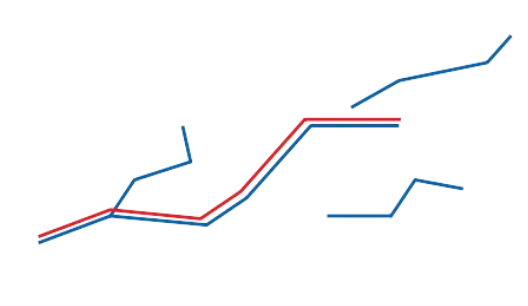
\includegraphics[width=1.00\textwidth]{nueselection/variables/trkfit.png}
    \caption{\label{fig:nue:variables:trkfit} ``trkfit'' variable }
    \end{subfigure}
    \begin{subfigure}[b]{0.3\textwidth}
    \centering
    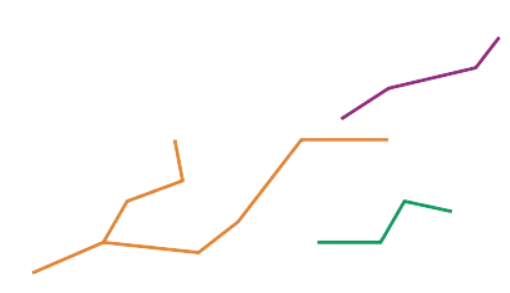
\includegraphics[width=1.00\textwidth]{nueselection/variables/nbranch.png}
    \caption{\label{fig:nue:variables:subcluster} ``subcluster'' variable }
    \end{subfigure}
    \begin{subfigure}[b]{0.3\textwidth}
    \centering
    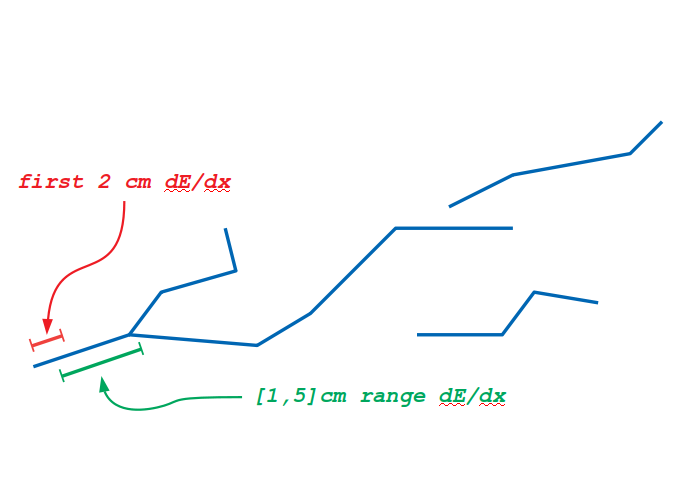
\includegraphics[width=1.00\textwidth]{nueselection/variables/dedx.png}
    \caption{\label{fig:nue:variables:dedx} d$E$/d$x$ variables }
    \end{subfigure}
\caption{\label{fig:nue:presel:eff} Additional shower variables defined by the analysis to improve track-shower separation.}
\end{center}
\end{figure}

\par \noindent  \textbf{Second Shower Based $\pi^0$ Rejection Variables}: Often in $\pi^0$ events one of the two EM $\gamma$ showers is not fully reconstructed by Pandora. In many cases, these second $\gamma$ showers are correctly identified by Pandora as belonging to the neutrino slice (reconstructed in 2D), but never fully reconstructed in 3D (see fig.~\ref{fig:nue:variables:secondshowerevd}). To improve on our $\pi^0$ rejection, we exploit this 2D-only information to reconstruct several variables which store information associated to the largest 2D cluster belonging to the slice on each plane. At the moment, only collection-plane variables are used. The variables, shown graphically in figure~\ref{fig:nue:variables:secondshower}, are described in table ~\ref{tab:variableSummary}. In the example event of figure~\ref{fig:nue:variables:secondshowerevd}, these quantities are computed for the circles black cluster of charge which represents a missed photon in the $\pi^0$ reconstruction.

\begin{figure}[H] 
\begin{center}
    \begin{subfigure}[b]{0.35\textwidth}
    \centering
    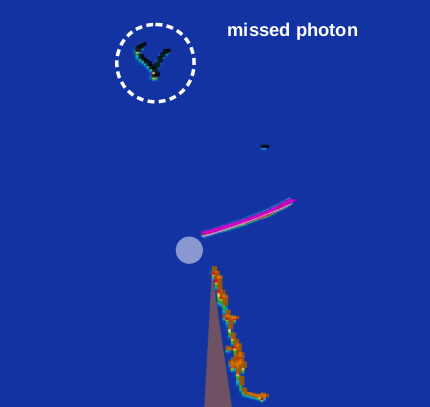
\includegraphics[width=1.00\textwidth]{nueselection/variables/secondshowerevd.png}
    \caption{\label{fig:nue:variables:secondshowerevd} unclustered shower }
    \end{subfigure}
    \begin{subfigure}[b]{0.35\textwidth}
    \centering
    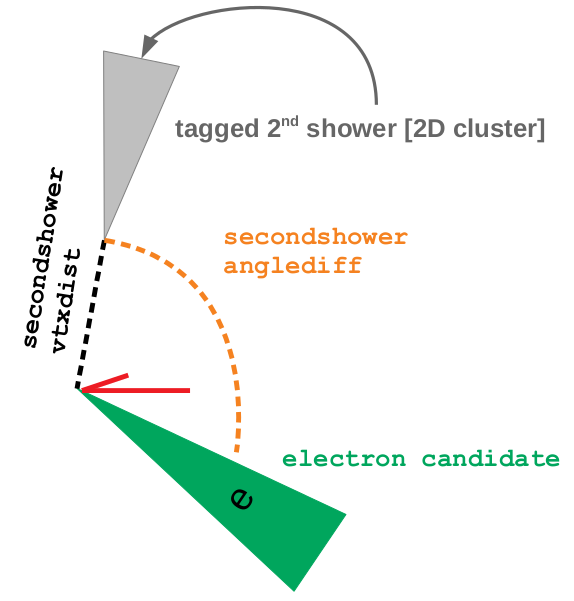
\includegraphics[width=1.00\textwidth]{nueselection/variables/secondshower.png}
    \caption{\label{fig:nue:variables:secondshower}second-shower variables }
    \end{subfigure}
\caption{\label{fig:nue:variables:secondshower} Visual representation of the second shower based $\pi^0$ rejection variables. Left: example event where the second shower in a $\pi^0$ event is clustered in 2D (black hits) but not fully reconstructed in 3D. Right: reconstructed variables associated to the 2nd-shower search. The gray cone in the image represents the black cluster on the left image, for which only 2D information is accessible.}
\end{center}
\end{figure}

\begin{table}[ht]
\caption{\label{tab:variableSummary} Summary of the definition for the variables used in the analysis.}
\centering
\begin{tabular}{ m{0.08\textwidth} | m{0.25\textwidth} | m{0.6\textwidth}  }
Category & Variable Name & Description  \\
\hline

\multicolumn{1}{l|}{} & \emph{nslice} &  Number of neutrino slices identified by the \emph{SliceID}. Values are  0 or 1.\\  \cline{2-3}
\multicolumn{1}{l|}{} & \emph{reco\_nu\_vtx\_sce\_\{x,y,z\}} & Reconstructed neutrino interaction vertex in (x,y,z) coordinates. The space charged correction is applied.  \\  \cline{2-3}
\multicolumn{1}{l|}{} & \emph{n\_showers\_contained} & Number of showers with a starting point within the fiducial volume. \\  \cline{2-3}
\multicolumn{1}{l|}{} & \emph{n\_tracks\_contained} & Number of tracks fully contained in the fiducial volume.  \\  \cline{2-3}
\multicolumn{1}{l|}{} & \emph{contained\_fraction} & Hits in PFParticles contained in the fiducial volume over the total number of clustered hits in the slice.  \\  \cline{2-3}
\parbox[t]{2mm}{\multirow{4}{*}{\rotatebox[origin=c]{90}{Slice}}} & \emph{hits\_ratio} & Ratio between hits from showers and total number of hits in the slice. \\  \cline{2-3}
\multicolumn{1}{l|}{} & \emph{CosmicIP} & Closest distance between shower start and space points associated to tracks flagged as cosmics. \\  \cline{2-3}
\multicolumn{1}{l|}{} & \emph{crtveto} & Boolean variable checking if the event passes the CRT veto. \\  \cline{2-3}
\multicolumn{1}{l|}{} & \emph{\_closestNuCosmicDist} &  3D distance between the reconstructed neutrino vertex and the closest CRT-tagged cosmic track. \\  \cline{2-3}
\multicolumn{1}{l|}{} & \emph{slclustfrac} & Fraction of hits in the slice that are fully reconstructed to 3D particles. \\  \cline{2-3}
\hline

\hline
\multicolumn{1}{l|}{} & \emph{trkpid}  &  Proton-muon LLR particle identification. \\  \cline{2-3}
\parbox[t]{2mm}{\multirow{4}{*}{\rotatebox[origin=c]{90}{Track, Shower and Their Separation}}}  & \emph{shr\_energy\_tot\_cali}  & Sum  of  the  energy  of  the  calibrated  showers  (in  GeV). Used  only  at pre-selection as a ``Michel veto”.\\  \cline{2-3}
\multicolumn{1}{l|}{} & \emph{shr\_score} & Pandora  SVM track/shower score for the leading shower.\\  \cline{2-3}
\multicolumn{1}{l|}{}  & \emph{tksh\_distance}  & Distance between leading shower and longest track start points.\\  \cline{2-3}
\multicolumn{1}{l|}{} & \emph{tksh\_angle}  & Angle  between  leading  shower   and  longest  track directions.\\  \cline{2-3}
\multicolumn{1}{l|}{} & \emph{merge\_bestdist}  & Distance between shower start point and track start (or end) point for the track in the slice that best matches the direction of the shower.\\  \cline{2-3}
\multicolumn{1}{l|}{} & \emph{trfit} & Fraction of the 3D spacepoints successfully fitted with the shower track-fitter algorithm. \\  \cline{2-3}
\multicolumn{1}{l|}{} & \emph{subcluster} & Number of isolated 2D segments of charge associated to a reconstructed shower on all three planes  \\  \cline{2-3}
\multicolumn{1}{l|}{} & \emph{shrmoliereavg} &  Average angle between the shower’s direction and its 3D spacepoints.    \\ \cline{2-3}
\multicolumn{1}{l|}{} & \emph{shr\_tkfit\_gap10\_dedx\_\{U,V,Y\}}  & Median dE/dx computed over the [1,5] cm of the shower’s  trunk. \\ \cline{2-3}
\multicolumn{1}{l|}{} & \emph{shr\_tkfit\_2cm\_dedx\_\{U,V,Y\}}  & Median dE/dx computed  over  the first 2 cm of the shower’s  trunk. \\ \cline{2-3}
\hline

\hline
\multicolumn{1}{l|}{} & \emph{secondshower\_Y\_nhit} & Number of hits in the collection plane of the largest cluster associated to the  recovered 2nd shower  \\  \cline{2-3}
\parbox[t]{2mm}{\multirow{4}{*}{\rotatebox[origin=c]{90}{Second Shower}}}  & \emph{secondshower\_Y\_dot} &  Dot product between the vector connecting the vertex to the closest hit in cluster and the charge-weighted cluster direction w.r.t. closest hit in cluster \\  \cline{2-3}
\multicolumn{1}{l|}{} & \emph{anglediff\_Y} & 2D angle difference in the collection plane between the 2nd shower and the 1st shower cluster  (cluster direction defined as charge-weighted direction of cluster w.r.t. vertex) \\ \cline{2-3}
\multicolumn{1}{l|}{} & \emph{secondshower\_Y\_vtxdist} & 2D distance from vertex for the largest 2D cluster associated to the  recovered 2nd shower in the collection plane \\
\hline
\end{tabular}
\label{tab:variableSummary}
\end{table}
